\renewcommand{\SourceFile}{6-geometrie-et-images/src/6-2.ml}

\section{Surface d'un polygone dessiné sur un réseau}

Soit $P$ un polygone dont toutes les arêtes sont horizontales ou verticales et tous les sommets à coordonnées entières. On le suppose donné par un mot décrivant son contour, de la façon suivante :\\
- on part de $(0,0)$\\
- on lit les lettres du mot une à une : \og d \fg{} signifie qu'on fait un pas d'une unité vers la droite, \og g \fg{} vers la gauche, \og h \fg{} vers le haut et \og b \fg{} vers le bas. Par exemple :
\medskip

\begin{center}
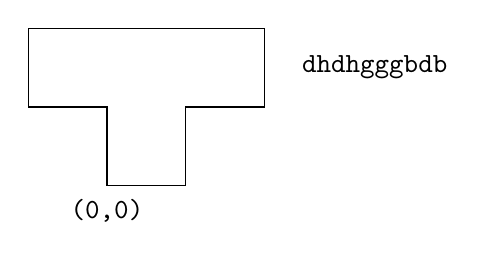
\begin{tikzpicture}[font=\ttfamily, label distance=-2pt]
    \node[label=below:{(0,0)}] at (0,0) {};

    \draw (0,0) -- (1,0) -- (1,1) -- (2,1) -- (2,2) -- (-1,2) -- (-1,1) -- (0,1) -- (0,0);

    \node at (3.4,1.5) {dhdhgggbdb};
\end{tikzpicture}
\end{center}

\Q
Écrire une fonction qui test si le polygone est fermé, c'est à dire si le dernier point du contour coïncide avec le premier.
\newpage

\Q
Écrire une fonction qui détermine les abscisses minimale et maximale $xmin$ et $xmax$ des points du polygone.

\Q
Soient $ymin$ et $ymax$ définis de façon similaire. On se donne une matrice d'entiers \texttt{t} de taille $n \times m$ initialement remplie par des 0. On veut \og dessiner \fg{} le polygone dans \texttt{t}, c'est à dire mettre des 0 et des 1 dans les entrées \texttt{t.(i).(j)} de façon que l'ensemble des entrées égales à 1 décrive le contour du polygone. Autrement dit, la matrice doit être comme une \og fenêtre \fg{} par laquelle on voit une portion de $\mathbb{Z}^2$. Écrire une fonction à cet effet.

\Q
Écrire une fonction pour calculer la surface du polygone.

\Q
Proposer une solution si le polygone est dessiné sur le réseau triangulaire (pavage du plan par des triangles équilatéraux) au lieu du réseau carré.

\Corrige

\Q
Il suffit de faire le tour du polygone à partir de $(0,0)$ en calculant à chaque pas la variation de l'abscisse et de l'ordonnée. On suppose le polygone donné par une chaîne de caractères.

\lstinputlisting[linerange={1-11}]{\SourceFile}

\Q
Là encore, il suffit de faire un parcours du contour en regardant à chaque pas la variation de l'abscisse et en mettant à jour \texttt{xmin} et \texttt{xmax} lorsque c'est nécessaire.
\newpage

\lstinputlisting[linerange={13-23}]{\SourceFile}

On supposera dans la suite disposer dans la suite d'une fonction \texttt{ordonnees} analogue.

\Q
Le polygone va pouvoir se tenir dans le tableau si et seulement si $xmax - xmin + 1$ et $ymax - ymin + 1$ sont tous deux inférieurs ou égaux à $n$. Attention à bien dessiner le contour tel qu'il apparaît dans $\mathbb{Z}^2$, et non une image de ce contour par rotation ou symétrie. En particulier, faire varier l'indice des lignes de la matrice de 0 à $n-1$ revient à faire varier l'ordonnée du point de $\mathbb{Z}^2$ de $ymax$ à $ymax-n+1$, et faire varier l'indice des colonnes de 0 à $n-1$ revient à faire varier l'abscisse du point de $\mathbb{Z}^2$ de $xmin$ à $xmin+n-1$. L'application qui à un point de $\mathbb{Z}^2$ associe une entrée de la matrice doit donc être :
\[
    \sigma : (x,y) \mapsto \texttt{t.(ymax-y).(x-xmin)}.
\]
Ainsi, $(0,0)$ a pour image \texttt{t.(ymax).(-xmin)}, et à chaque lettre lue on a :\\
\og d \fg{} : \texttt{j} augmente de 1\\
\og g \fg{} : \texttt{j} diminue de 1\\
\og h \fg{} : \texttt{i} diminue de 1\\
\og b \fg{} : \texttt{i} augmente de 1.\\
D'où la fonction :

\lstinputlisting[linerange={37-57}]{\SourceFile}

\Q
Le calcul de la surface $A$ peut sembler difficile, mais en fait il suffit d'utiliser la formule de Green-Riemann (cas particulier de la formule de Stokes) pour que la programmation devienne très simple.
